%*******************************************************************************
%*******************************************************************************
\chapter{Songbook}
\setcounter{chapter}{1}
\label{chap:songbook}
\minitoc
\fancyhead[RE]{\textit{Chapitre \arabic{chapter}.~\nouppercase{\leftmark}}}
\fancyhead[LO]{\textit{\arabic{chapter}.\arabic{section}.~\nouppercase{\rightmark}}}
%*******************************************************************************
%*******************************************************************************


%*******************************************************************************
\section{Setup}
\label{sec:install}
%*******************************************************************************

Globally, avoid any file/directory name with spaces or special
characters. In this guide, we consider that the working directory is:
\directory{\$HOME/songbook} which may also be referred to as
\directory{/home/user/songbook} or \directory{$\sim$/songbook}.

%------------------------------------------------------------------------------
\subsection{\linux}
%------------------------------------------------------------------------------

A songbook uses \LaTeX{} to render the songs' layout and Python to
generate indexes (required dependencies). Music sheets can be included
if written with Lilypond and source code is hosted/distributed as a
\git repository (recommended dependencies). Finally, a pdf reader
application is required to open produced songbooks. For Debian/Ubuntu
users~:

\paragraph{Dependencies}

Install required dependencies.
\begin{unix}
  sudo apt-get install texlive-base texlive-latex-extra
  sudo apt-get install texlive-lang-french python
\end{unix}

Install recommended dependencies.
\begin{unix}
  sudo apt-get install texlive-fonts-recommended
  sudo apt-get install lilypond
\end{unix}

\paragraph{Sources}

Sources can be retrieved as a \ext{tar.gz} archive
\begin{unix}
  wget http://www.patacrep.com/data/documents/songbook.tar.gz
  tar xzvf songbook.tar.gz
\end{unix}

or as a \git repository

\begin{unix}
  git clone git://git.lohrun.net/songbook.git
\end{unix}

\paragraph{Compile and run}

The compilation chain is automated through a \emph{makefile}. In your
songbook's directory:

\begin{unix}
  make all
\end{unix}

Some makefile's options:
\begin{itemize}
\item \command{\$ make clean}~: removes logs and temporary files
  produced during the compilation step, except \ext{pdf} files.
\item \command{\$ make cleanall}~: removes all temporary files and
  produced \ext{pdf}.
\item \command{\$ make lilypond}~: generates music sheets
  corresponding to Lilypond sources (\ext{ly} files) as \ext{pdf} in
  \directory{./lilypond}. The Lilypond software is required.
\item \command{\$ make book.pdf}~: since \command{make} or
  \command{make all} may take some time, if you are only interested in a
  single songbook, you can specify the book (\ext{ext}) you
  want. Instead of \file{book.pdf}, you may choose:
\end{itemize}

\begin{center}
  \begin{tabular}{l l}
    \hline
    \command{make} & description \\
    \hline
    \file{songbook.pdf} &~: full version with the whole set of songs and music sheets \\
    \file{volume-1.pdf} &~: volume 1 (171 songs, 152 pages)\\
    \file{volume-2.pdf} &~: volume 2 (180 songs, 157 pages) \\
    \file{naheulbeuk.pdf} &~: a songbook for the \emph{Donjon de Naheulbeuk}\\
    \file{english.pdf} &~: english songs only\\
    \file{french.pdf} &~: french songs only\\
    \hline
  \end{tabular}
\end{center}

Note that the \command{make} command without any option corresponds to
\command{make \file{songbook.pdf}}.

%------------------------------------------------------------------------------
\subsection{\windows}
%------------------------------------------------------------------------------

\paragraph{Dependencies}

Install required dependencies.
\begin{itemize}
\item Miktex~: \url{http://miktex.org/}
\item Python~: \url{http://www.python.org/download/releases/2.7.2/}
\end{itemize}

\begin{nota}
The compilation process under \windows has been tested with MikTeX~2.9
and Python~2.7.2.
\end{nota}

Install recommended dependencies.
\begin{itemize} 
\item Lilypond~: \url{http://lilypond.org/install/}
\end{itemize}


\paragraph{Modify the \command{Path} variable}

Restart your computer after installing MikTeX and Python. The
\command{Path} variable now needs to be modified.
\begin{itemize}
\item Right-click on My Computer, then Properties.
\item In \menu{Parameters}{Advanced Settings}, click on Environment
  Variables.
\end{itemize}

In the lower part (System Variables), scroll the list until the
\command{Path} command, then double-click to modify. The \command{Path}
contains a set of paths that are separated by semicolons. The
following paths must be present:
\begin{itemize}
\item Python~: \verb#C:\textbackslash Python27#
\item Miktex~: \verb# C:\Program Files\MiKTeX 2.9\miktex\bin#
\item Lilypond~: \verb#C:\Program Files\LilyPond\usr\bin#
\end{itemize}

\begin{nota}
Pay attention to version numbers. These directories are just examples
that may need to be adapted according to your downloaded software
version.
\end{nota}

Restart your computer once your \command{Path} is modified.

\paragraph{Sources}

Sources can be retrieved as a \ext{tar.gz} archive at
\url{http://www.patacrep.com/data/documents/songbook.tar.gz}. Its
content can be extracted with third-party softwares such as
7zip\footnote{\url{http://www.7-zip.org/}} or
Winrar\footnote{\url{http://www.win-rar.com/}}.

Alternatively, in the case you have installed a
Git\footnote{\url{http://git-scm.com/}} client, for instance
Mysysgit\footnote{\url{http://code.google.com/p/msysgit/}}, you can
download the sources with:

\begin{unix}
  git clone git://git.lohrun.net/songbook.git
\end{unix}

\paragraph{Compile and run}

\begin{enumerate}
\item Open the command prompt~: \Key{Windows}+\Key{r}, enter
  \command{cmd} and validate with \Key{Enter}
  (\reffig{fig:terminal-windows}).
\item Go to the songbook directory using \command{cd}.
For instance,
  \begin{unix}
    cd C:\
    cd songbook
  \end{unix}
\item Use the file \file{make.bat}, giving a \ext{sb} file as parameter.
  For instance,
  \begin{unix}
    make.bat songbook.sb
  \end{unix}
\end{enumerate}

\begin{nota}
MikTeX is a \LaTeX{} distribution that allows to install missing
packages {\og}on the fly{\fg}. A songbook usually requires a few
additional packages (\reffig{fig:paquets-miktex}).
\end{nota}

%*******************************************************************************
\section{Content description}
\label{sec:contents}
%*******************************************************************************

\paragraph{\directory{./utils}}
\label{sec:utils}
Contains a set of scripts. To run a script, enter the following command in a terminal:

\begin{unix}
  ./utils/script.sh
\end{unix}

\begin{itemize}
\item \file{resize-cover.sh}~: automatically resize \ext{jpg} files of
  the \directory{songbook/songs} directory. Those files correspond to
  songs' covers. Run this script after introducing a new jpg cover.

\item \file{rules.py}~: apply a set of rules for \LaTeX{} specific
  notations or chords. Run this script after adding a new song or
  after modifying an existing one in order to preserve global songbook
  standards.

\item \file{typo.sh}~: apply a set of typographical rules such as the
  removal of double/trailing spaces or language specific rules. Run
  this script after adding a new song or after modifying an existing
  one in order to preserve global songbook standards.

\item \file{new-songs-list.sh}~: allows to retrieve the list of songs
  that have been added since the last release.

\item \file{make-html.sh}~: builds an html index for the whole set of
  songs.
\end{itemize}

\paragraph{\directory{./templates}}
Contains some files corresponding to different songbook styles.  A
template contains some parameters such as the font size, color
settings etc.

\begin{itemize}
\item \file{patacrep.tmpl}~: default template.
\item \file{patacrep-en.tmpl}~: english version of the default
  template.
\item \file{minimal.tmpl}~: a more compact version without front page
  nor indexes.
\end{itemize}

%%%%%%%%%%%%%%%%%%%%%%%%%%%%%% FIGURE %%%%%%%%%%%%%%%%%%%%%%%%%%%%%%%%%%
\begin{figure}
  \centering
  %% -- subfigures --
  \subfigure[]{
    \label{fig:templates-a}
    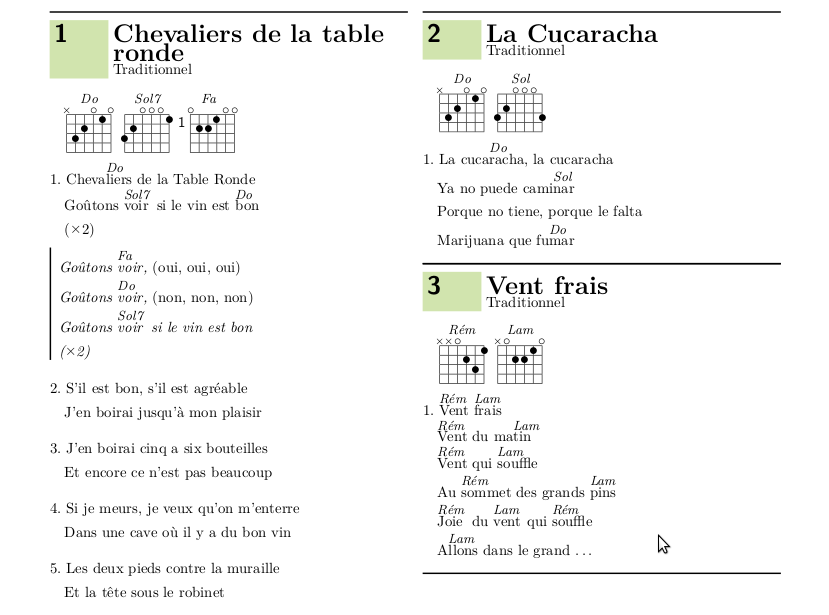
\includegraphics[width=0.35\textwidth]{templates-a}%
  }%
  \hspace{0.1cm}%
  \subfigure[]{%
    \label{fig:templates-b}%
    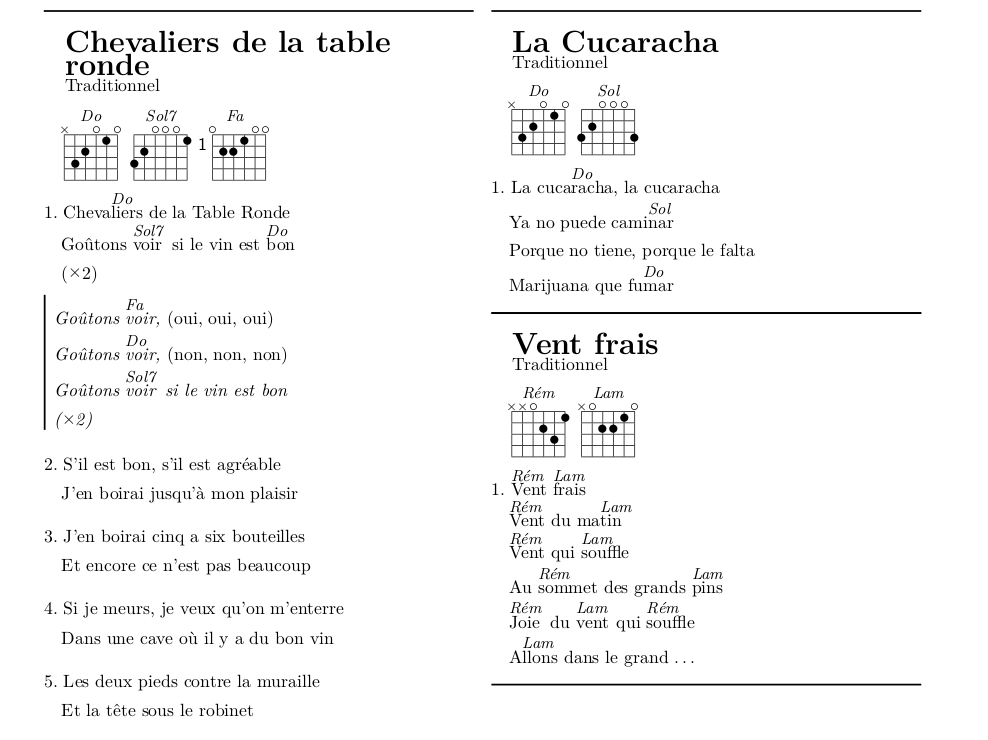
\includegraphics[width=0.35\textwidth]{templates-b}%
  }%
  %% -- subfigures --
  \caption[Templates]{% 
    Different templates may be used for a same songbook.
    \subref{fig:templates-a}~Template \file{patacrep.tmpl}; % 
    \subref{fig:templates-b}~Template \file{minimal.tmpl}.%
  }%
  \label{fig:templates}
\end{figure}
%%%%%%%%%%%%%%%%%%%%%%%%%%%%%%%%%%%%%%%%%%%%%%%%%%%%%%%%%%%%%%%%%%%%%%%%


\paragraph{\directory{./songs}}
Contains the set of available songs. Each song is a text file with the
\ext{sg} extension. A song is found in a sub-directory named by the
corresponding artist. For instance:
\file{songs/Pornophonique/Sad\_robot.sg}.

\paragraph{\directory{./lilypond}}
Contains the Lilypond music sheet sources as \ext{ly} files.

\paragraph{\directory{./tex}}
Contains a few additional \LaTeX{} files such as packages, licenses etc.

\paragraph{\directory{./img}}
Contains the images that may be inserted in a songbook (except album
covers). To add the image \file{my\_image.jpg} in a song, use the
\latexcom{image} macro inside a \ext{sg} file. This macro behaves like
the \LaTeX{} macro \latexcom{includegraphics}. For example:

\begin{songbook}
  \image[width=4cm]{my\_image}
\end{songbook}

%*******************************************************************************
\section{Start a new songbook}
\label{sec:create-songbook}
%*******************************************************************************

In order to build a songbook, a \ext{sb} file is required whose
content is detailed in the following. A songbook file (\ext{sb})
contains a set of values for the options that are provided by a
template and a list of songs.  A \ext{sb} file must be saved at the
root of the project. Following is an example of a songbook file based
on the minimal template and containing two songs.

\begin{code}
{
"template" : "minimal.tmpl",
"bookoptions" : [
    "diagram",
    "lilypond",
    "pictures"
  ],
"songs" : [
    "Le_Donjon_de_Naheulbeuk/10_sous_dans_ma_poche.sg",
    "Le_Donjon_de_Naheulbeuk/Bugger_off.sg"
  ]
}
\end{code}

Available options are defined in the template file. In this case, the
value \emph{["diagram", "lilypond", "pictures"]} has been set for the
option \emph{bookoptions} of the \file{minimal.tmpl} template.
Using the \file{patacrep.tmpl} template, the following options are available:

\begin{center}
  \rowcolors{1}{white}{Aluminium1}
  \begin{tabular}{l l l}
    \hline\noalign{\smallskip}
    Option & Description  & Type \\
    \noalign{\smallskip}
    \hline
    \noalign{\smallskip} 
    title & songbook title & character string \\
    author & songbook authors & character string \\
    booktype & whith/without chords & \command{chorded} or \command{lyric}\\
    bookoptions & display elements & \command{diagram}, \command{lilypond},\\
    & & \command{pictures}, \command{tabs}\\
    version & current pdf version & character string \\
    subtitle & songbook subtitle & character string \\
    web & Internet website & character string \\
    mail & contact email & character string \\
    picture & front page picture & path to image file\\
    & & \ext{png}, \ext{jpg} or \ext{pdf}\\
    picturecopyright & picture copyright & character string \\
    footer & front page footer & character string \\
    license & document license & character string \\
    mainfontsize & document font size & 10, 11 or 12 pt\\
    songnumberbgcolor & songs number background color & hexadecimal color code \\
    notebgcolor & textnote background color & hexadecimal color code \\
    indexbgcolor & color of indexes' links & hexadecimal color code \\
    \hline
  \end{tabular}
\end{center}

Once your songbook \file{mybook.sb} is written, produce the corresponding pdf with:
\begin{unix}
make mybook.pdf
\end{unix}


%*******************************************************************************
\section{Writing a song}
\label{sec:write-song}
%*******************************************************************************

%------------------------------------------------------------------------------
\subsection{Main elements}
%------------------------------------------------------------------------------

A song is a plain text file \file{song.sg} that is saved in a
\directory{songs/Artist} directory. Remember that filenames do not
accept spaces (replace them with underscores). A \ext{sg} file header
is composed of the following elements~:

\begin{songbook}
\beginsong{Title}
  [by=<Artist>,cov=<album-cover>,album=<Album>]
\end{songbook}

The \command{Title}, \command{Artist}, \command{album-cover} and
\command{Album} parameters must be set for each new song. The field
\command{album-cover} denotes a file \file{album-cover.jpg} that is in
the same directory of the corresponding \ext{sg} song. 

A song is a sequence of verses and chorus. Use the macros
\latexcom{beginverse} and \latexcom{endverse} to determine the text of
a same verse. Similarly, use the macros \latexcom{beginchorus} and
\latexcom{endchorus} for the text of a same chorus.

To insert a guitar chord in the text, a special command is used. For
instance, the \latexcom{[E]} command will print the chord \command{E}
above the following syllable in the pdf.

\begin{songbook}
\beginverse
  His \[Dm]steely skin is covered
  By \[F]centuries of dust
  \[C]Once he was a great one
  \[Dm]Now he's dull and rust
\endverse
\end{songbook}

A song ends with the macro \latexcom{endsong}.

%------------------------------------------------------------------------------
\subsection{Style guidelines}
%------------------------------------------------------------------------------

\paragraph{Chords notation}
Chords follow the British/American notation (A, B, C, D, E, F, G). By
default, the chord is major (C refers to C major). Minor chords are
written with a lower-case \command{m}. The flat symbol ($\flat$) is
obtained with the symbol \command{\&}. The sharp symbol ($\sharp$) is
obtained with the character \command{\#}. For example, the
\command{A flat minor} chord is written \latexcom{[A\&m]}.

\paragraph{Repeating chords}
In order to maintain an easy to read and compact document, chords in
verse and chorus are only specified once. This may be harder to
decipher the first time but in the end, the text is much more easier
to read and that's a lot less of pages to print.

\paragraph{Typography}
\begin{itemize}
  \item Each line begins with a capital letter;
  \item No punctuation (except ``! or ?'') at the end of lines;
  \item Symbols such as {\og}; : ! ?{\fg} require an unbreakable space
    before in French but not in English~;
  \item French capital letters are accentuated (e.g {\og}À bientôt{\fg}
    and not {\og}A bientôt{\fg}).
\end{itemize}

\paragraph{Verse numbering and line breaks}
The numbering is automatically performed and increased with each new
\latexcom{beginverse} environment. However, it is often convenient to
decompose a same verse in two parts, without numbering the second
part. To achieve this, use the \latexcom{beginverse*} macro. For
instance, a verse composed of eight verses (lines) may usually be
decomposed in two verses of four lines. For example:

\begin{songbook}
\beginverse
  His \[Dm]steely skin is covered
  By \[F]centuries of dust
  \[Do]Once he was a great one
  \[Dm]Now he's dull and rust
\endverse

\beginverse*
  An oily tear he's crying
  Can you feel the pain
  Of the sad, sad robot
  And it's driving him insane
\endverse
\end{songbook}

\paragraph{Columns layout}
The macro \latexcom{songcolumns} determines the number of columns of
the song in the final pdf. Use this macro right before the
\latexcom{beginsong} command. Usually, a song is presented on 1, 2 or
3 columns. By default, specify two columns.

\begin{songbook}
\songcolumns{2}
\beginsong{Title}
\end{songbook}

\paragraph{Special characters}
A few characters must be written according to \LaTeX{} commands for a
better rendering in the pdf. For example, ellipsises should be written
by the command \latexcom{dots}. See also \refsec{sec:utils}.

\paragraph{Echo and repeat}
When a sentence is repeated several times, use the command
\latexcom{rep} instead of writing \emph{bis} or (x4). For example, if the
word \emph{Hallelujah} is repeated four times, write:

\begin{songbook}
Hallelujah \rep{4}
\end{songbook}

The command \latexcom{echo} refers to choirs or alike.

\begin{songbook}
Hallelujah \echo{Hallelujah}
\end{songbook}

\paragraph{Chords diagrams}
Given that the same guitar chord may be played differently and that
one position may be better than another, the songbook allows to
represent the chord as a diagram at the beginning of the song through
the command \latexcom{gtab}, right before the first verse of the
song. Following are a few examples:

\begin{songbook}
\gtab{C}{3:002220}
\gtab{D}{XX0232}
\gtab{E}{022100}
\gtab{Am}{X02210}
\end{songbook}

\begin{nota}
  \begin{itemize}
  \item X is the capital letter x. The lower-case variant is not supported.
  \item 0 is the figure zero and not the capital letter O.
  \end{itemize}
\end{nota}

\begin{itemize}
\item the six figures correspond to the six guitar strings
  (\chord{E}, \chord{A}, \chord{D}, \chord{G},
  \chord{B}, \chord{E})~;
\item the value indicates the fret to be played;
\item 0 denotes an open string;
\item X indicates that the string should not be played;
\item a value before ``:'' denotes a barre (\emph{3:} denotes a barre chord on third fret).
\end{itemize}

%------------------------------------------------------------------------------
\subsection{Lilypond music sheets}
%------------------------------------------------------------------------------

If you want to add a melodic pattern in a song, you may use Lilypond
syntax to write the score. In this regard, open a new file
\file{score.ly} in the repertory \directory{songbook/lilypond}.
Import the file \file{header} at the beginning of your file and define
the option \command{paper-height} to ensure that the pdf score fits
one single page with minimum whitespace. A first approach is to count
1.6\,cm for a single line. Then, write your score between brackets
(see~\reffig{fig:lilypond}).

%%%%%%%%%%%%%%%%%%%%%%%%%%%%%%%% FIGURE %%%%%%%%%%%%%%%%%%%%%%%%%%%%%%%%%%%%%%%%%
\begin{figure}
  \begin{minipage}[b]{\linewidth}
    \centering
    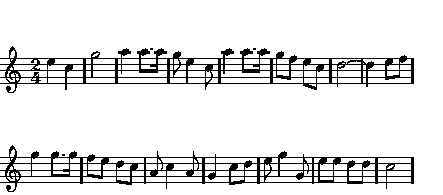
\includegraphics[width=0.8\textwidth]{lilypond}
    \vspace{0.5cm}
  \end{minipage}

  \begin{minipage}[b]{\linewidth}
\begin{lilypond}
\include "header" 
\paper{paper-height = 3.3\cm} 
{
  \key c \major 
  \time 2/4 
  \relative c''
    {
      e4 c g'2 a4 a8. a16 g8 e4 c8 
      a'4 a8. a16 g8 f e c d2~ d4 
      e8 f g4 g8. g16 f8 e d c a c4 a8 g4 
      c8 d e8 g4 g,8 e' e d d c2
    } 
}
\end{lilypond}
  \end{minipage}
  \caption{Source code for a Lilypond music sheet.}
  \label{fig:lilypond}
\end{figure}
%%%%%%%%%%%%%%%%%%%%%%%%%%%%%%%%%%%%%%%%%%%%%%%%%%%%%%%%%%%%%%%%%%%%%%%%%%%%%%%%

Finally, your file \file{sheet.ly} can be inserted in a song \ext{sg} through
the \latexcom{lilypond} command:

\begin{songbook}
\lilypond{sheet}
\end{songbook}

%------------------------------------------------------------------------------
\subsection{Example}
%------------------------------------------------------------------------------

Here is a complete example of the song \emph{Sad robot} by
\emph{Pornophonique}\footnote{\byncnd~\url{http://www.jamendo.com/fr/track/81740}}
that may be used as a reference for a new song.

\begin{songbook}
\selectlanguage{english}
\songcolumns{2}
\beginsong{Sad robot}
  [by=Pornophonique,cov=8-bit-lagerfeuer,album=8-bit lagerfeuer]

  \cover
  \gtab{Dm}{XX0231}
  \gtab{F}{1:022100}
  \gtab{C}{X32010}

  \lilypond{Sad_robot}

  \beginverse
    His \[Dm]steely skin is covered
    By \[F]centuries of dust
    \[C]Once he was a great one
    \[Dm]Now he's dull and rust
  \endverse

  \beginverse*
    An oily tear he's crying
    Can you feel the pain
    Of the sad, sad robot
    And it's driving him insane
  \endverse

  \beginverse*
    He can't turn back time nor history
    So his life became a misery
    He has to face the destiny
    Nobody cares anymore
  \endverse

  \beginchorus
    Sad, sad robot
    Sad, sad robot
    Sad, sad robot
    All alone
  \endchorus

  \beginchorus
    He's a sad, sad robot \rep{3}
    He's so alone
  \endchorus

  \beginverse
    Me steely skin is covered
    By centuries of dust
    Once me was a great one
    But now I'm dull and rust
  \endverse

  \beginverse*
    An oily tear I'm crying
    Can you feel me pain
    I'm the sad, sad robot
    Driving me insane
  \endverse

  \beginverse*
    I can't turn back time nor history
    So me life became a misery
    I have to face me destiny
    That I'm all on me own
  \endverse

  \beginchorus
    Red, red robot
    I'm a red, red robot \rep{2}
    And so I shall return
  \endchorus

  \beginchorus
    I'm a red, red robot \rep{3}
    So I shall return
  \endchorus
\endsong
\end{songbook}
